\section{Einleitung}
%Kontext
In Zusammenarbeit mit dem Spezialisten für Konserventechnik, der Ferrum AG, entwickelt die Fachhochschule Nordwestschweiz FHNW einen neuen Dosenverschliesser für die Getränke- und Lebensmittelindustrie. Dieser soll hauptsächlich kleinere Unternehmen ansprechen mit begrenztem Budget und geringeren Anforderungen hinsichtlich dem Durchsatz. Um eine Dose zu verschliessen, sind auf einem Drehteller vier Motoren mit den dazugehörigen Werkzeugen angeordnet, um die notwendigen Arbeitsschritte durchzuführen. Durch die FHNW wurde bereits ein erster Aufbau der Maschine realisiert. In diesem ersten Aufbau werden die vier Motoren-Drives mit einer Schleppkette versorgt, welche die Kabel für Energieversorgung und Datenkommunikation führt. Eine Schleppkette ist wartungsintensiv und sperrig und deshalb für eine industrielle Anlage ungeeignet.
\newline
\ \\
%Ziel+Anforderungen
In dieser Projektarbeit soll eine berührungslose Energie- und Datenübertragung auf den Drehteller realisiert werden. Folglich würden die Kabel und die lange Schleppkette ersetzt werden. Die vier Motoren brauchen zusammen eine Leistung von mindestens $\SI{300}{W}/\SI{48}{V}$. Die Datenübertragung funktioniert über einen VARAN Ethernet-Bus. Ziel im Projekt 5 ist es, möglichst viele Erkenntnisse zur berührungslosen Energie- und Datenübertragung zu sammeln und daraus die richtigen Schlüsse zu ziehen. Mit diesem, im Projekt 5 ausgearbeiteten Konzept, wird die Vorarbeit für die Bachelor-Thesis im Projekt 6 geleistet. Dort soll schliesslich ein Produkt entstehen, welches im Dosenverschliesser die Schleppkette ersetzen kann.
\newline
\ \\
%Lösungsansätze
Die Energieübertragung wird induktiv über zwei Spulen mit Ferrit-Kern realisiert. Dafür wurden mehrere Simulationen durchgeführt, um die beiden Spulen zu dimensionieren. Für die Ansteuerung der Spulen wurden einige gängige Schaltungstypen simuliert und schliesslich eine Testschaltung aufgebaut. Die Daten sollen mittels optischer Übertragung auf den Drehteller und zurück gesendet werden. Dafür wurden infrarot Emitter, Photodioden und Transimpedanzverstärker evaluiert und simuliert. Schliesslich wurde eine Testschaltung entworfen, um herauszufinden, ob die notwendige Geschwindigkeit erreicht werden kann. Für eine störungsarme Übertragung, sind zwei optisch getrennte Kanäle vorgesehen.
\newline
\ \\ 
%Aufbau der Arbeit
Die Energieübertragung und die Datenübertragung konnte im Projekt 5 separat untersucht werden. Dementsprechend ist dieser Bericht auch aufgebaut. Im Kapitel \ref{sec:Grundlagen} \nameref{sec:Grundlagen} werden die wichtigsten Theorien und Erklärungen für die weiteren Teile des Berichts geliefert. Die \nameref{sec:energie} wird im Kapitel \ref{sec:energie} vom Konzept bis zur Validierung des Testaufbaus detailliert dargelegt. Im Kapitel \ref{sec:Daten} \nameref{sec:Daten} wird alles vom Konzept der Sender- und Empfängerschaltung bis zur Validierung beschrieben. Das Kapitel \ref{sec:Fazit} \nameref{sec:Fazit} fasst die wichtigsten Erkenntnisse aus dem Bericht zusammen und beschreibt die Ausgangslage für das Projekt 6.


%\begin{figure}
%\centering
%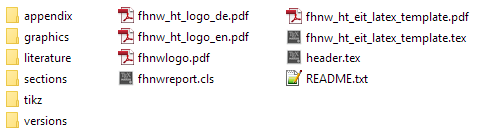
\includegraphics[width=0.8\linewidth]{ordner_struktur.png}
%\caption{Minimalstruktur des \LaTeX -Projekts.}\label{fig:Struktur}
%\end{figure}

